\documentclass[a4paper]{article}
\usepackage{enumitem}
\usepackage[utf8]{inputenc}
\usepackage{amsmath}
\usepackage{mathtools}
\usepackage{hyperref}
\usepackage{graphicx}
\usepackage{float}
\DeclarePairedDelimiter{\floor}{\lfloor}{\rfloor}

\title{Assignment 1}
\author{Mytraya Gattu, 180050032}
\date{22 August 2020}
\begin{document}
\maketitle
\section{Problem 1}
In what follows, $r$ is the radius of the hemispherical caps,$l$ the length and $m$ of the cell. It is given that, 
$$r=0.5\mu \text{m}$$
$$l=2\mu \text{m}$$
\begin{enumerate}[label=(\alph*)]
  \item Volume is given by $$V=\pi r^2 l + \frac{4}{3}\pi r^{3} = 2.094 \mu \text{m}^{3}$$
  Typical cell volume is $0.6-0.7 \mu \text{m}^{3}$
  \newline
  \url{https://en.wikipedia.org/wiki/Escherichia_coli}
  \item $m$ is the sum of the mass of water contained and that of the other substances. Since, density of water is $$10^3 \frac{\text{kg}}{\text{m}^3}=10^{-6} \frac{\text{pg}}{\mu \text{m}^3}$$
  We have
  $$m=10^{-6} \cdot \left(\frac{2}{3} + 1.3\cdot \frac{1}{3}\right)\cdot V \text{pg} = 2.304 \cdot 10^{-3} \text{pg}$$
  
  Typical cell weight is $1\cdot 10^{-3} \text{pg}$ \newline \url{https://ecmdb.ca/e_coli_stats)}
\end{enumerate}
It is evident from the above calculations, that the it is the assumed shape of \textit{E. coli} which deviates greatly from what is true. 
\pagebreak 
\section{Problem 2}
    Let at the end of $9^{\text{th}}$ cycle there be $N$ nuclei at the surface. At the end of $13^{\text{th}}$ cycle, therefore there are $16N$ nuclei, which is given as $\approx 6000$. Hence, $$N \approx 375$$
    Since, every embryo must start from a single fertilized nucleus, at the end of $9^{\text{th}}$ cycle, there must be $2^{9} = 512$ nuclei in total. Therefore, the fraction of nuclei which migrated to the surface is$$\frac{375}{512} \approx 0.7324$$
    Following the notation of Problem 1, surface area of the spherocylinder is $$A=4\pi r^{2} + 2\pi r l = 4.3982\cdot 10^{-7} \text{m}^{2}$$ 
    Therefore, the areal density is $$1.3642\cdot10^{10} \frac{\text{nuclei}}{\text{m}^2}$$
    (For the next part, I have used Mathematica.)
    To calculate the length of the green strips, I marked the ends of widths along the lenghts of each strip, and then used the given scale.
    \begin{figure}
    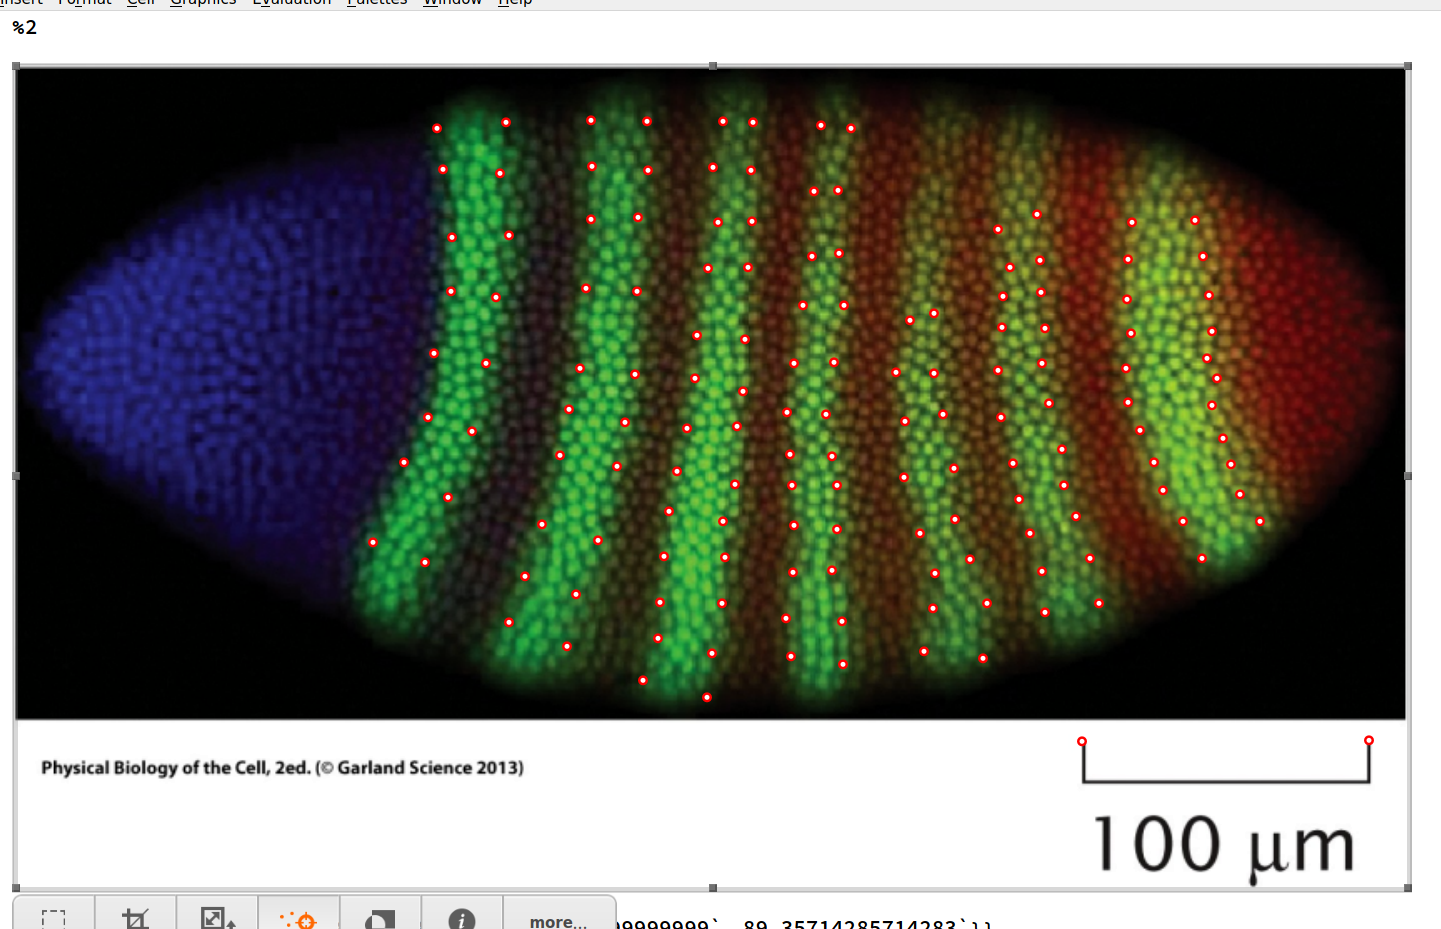
\includegraphics[width=10cm]{q2_length.png}
    \centering 
\end{figure} \newline
    Length of the green strip is: $18.37 \pm 4.99 \mu \text{m}$
    To evaluate the number of nuclei in each strip, I isolated the colors, and counted the number of pixels.
    \begin{figure}
        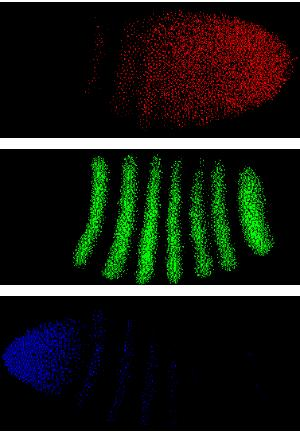
\includegraphics{q2_count.jpeg}
    \centering 
\end{figure} \newline
    Therefore, the number of nuclei corresponding to each dye(I'm considering only a single surface)
    \begin{itemize}
        \item Red: 148
        \item Green: 210
        \item Blue: 58
    \end{itemize}
\pagebreak
\section{Problem 3}
\subsection{E. coli}
Mean of sequence length: $1892.00$ \newline
Standard deviation of sequence length: $3872.73$ \newline
Mean of molecular mass: $289.03$ \newline
Standard deviation of molecular mass: $775.76$ \newline
\subsection{S. cerevisiae}
Mean of sequence length: $1287.90$ \newline
Standard deviation of sequence length: $2444.49$ \newline
Mean of molecular mass: $154.78$ \newline
Standard deviation of molecular mass: $313.31$ \newline
\subsection{Humans}
Mean of sequence length: $630.74$ \newline
Standard deviation of sequence length: $1263.08$ \newline
Mean of molecular mass: $74.21$ \newline
Standard deviation of molecular mass:$181.93$ \newline
\begin{figure}
    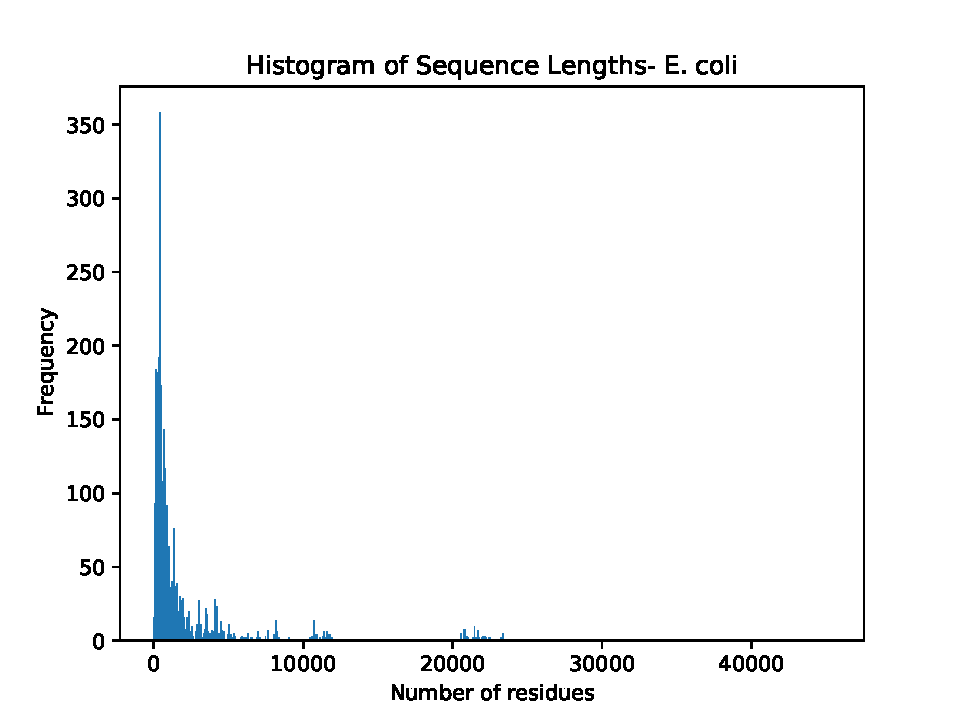
\includegraphics{ecoli_length.pdf}
\centering 
\end{figure} 
\begin{figure}
    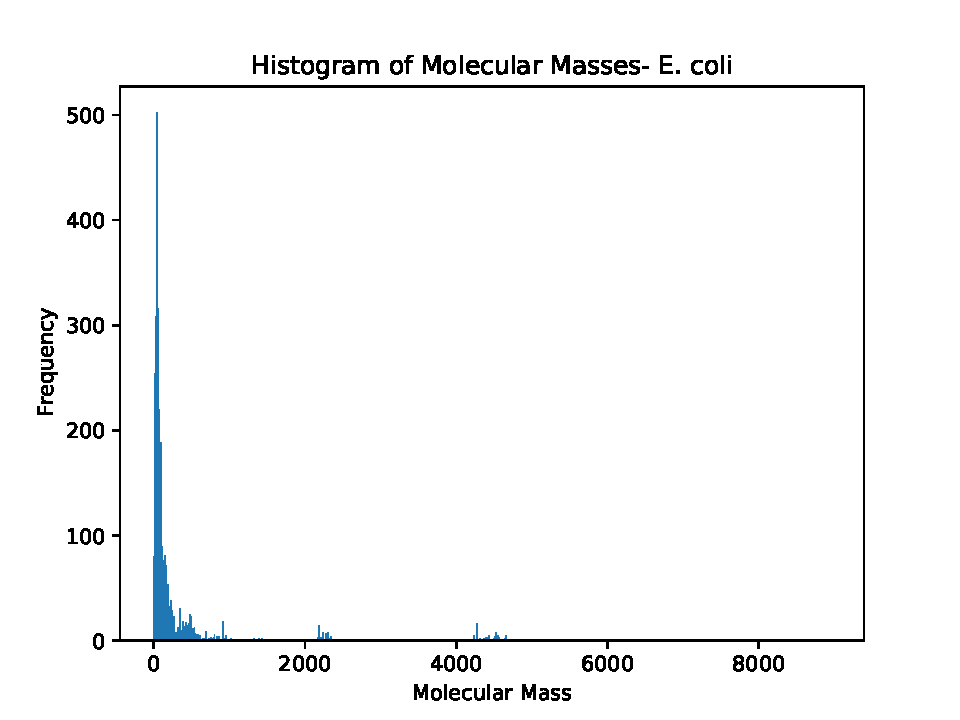
\includegraphics{ecoli_mass.pdf}
\centering 
\end{figure} 
\begin{figure}
    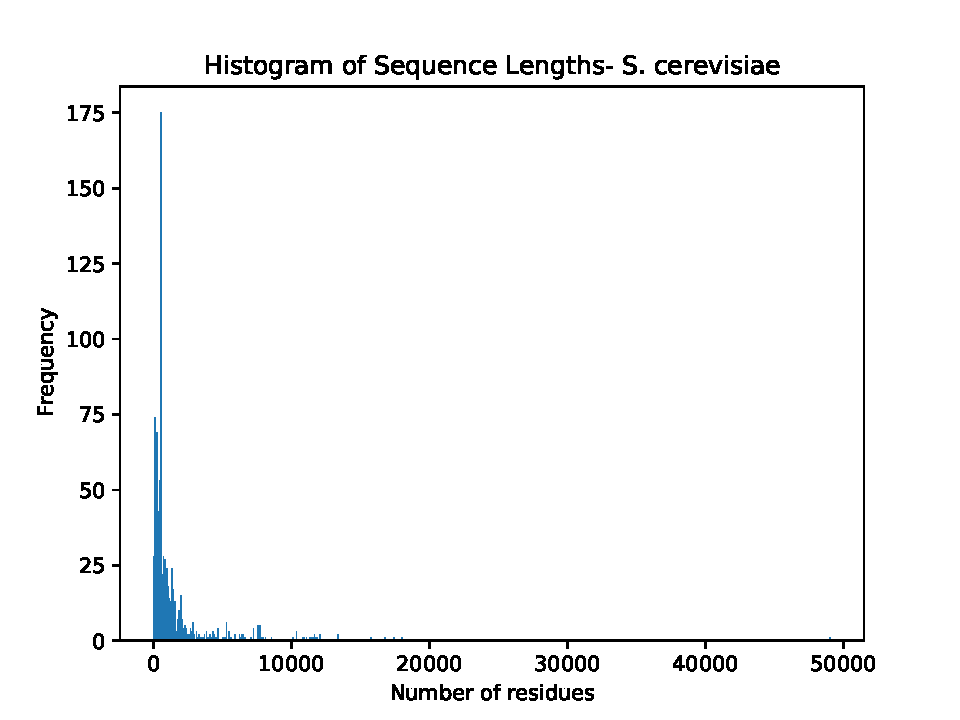
\includegraphics{scerevisiae_length.pdf}
\centering 
\end{figure} 
\begin{figure}
    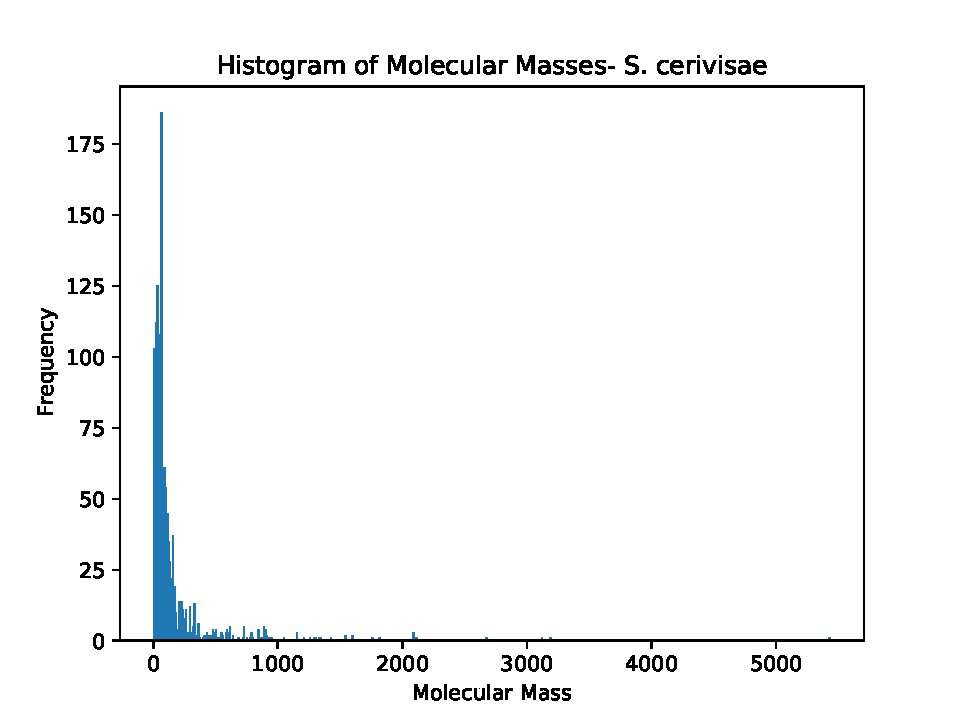
\includegraphics{scerevisiae_mass.pdf}
\centering 
\end{figure}
\begin{figure}
    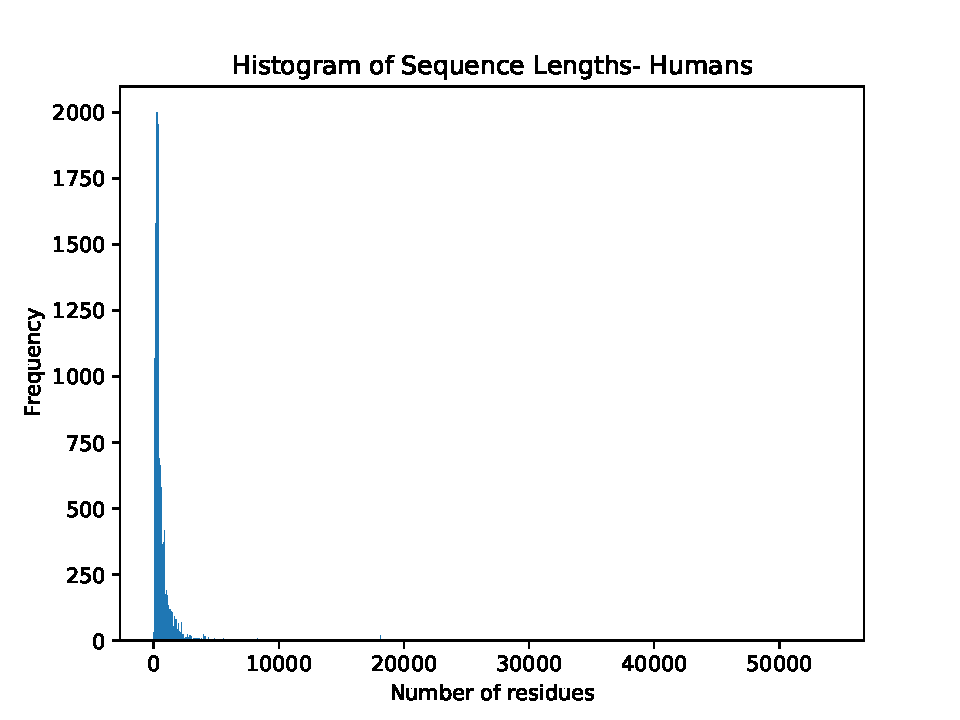
\includegraphics{human_length.pdf}
\centering 
\end{figure} 
\begin{figure}
    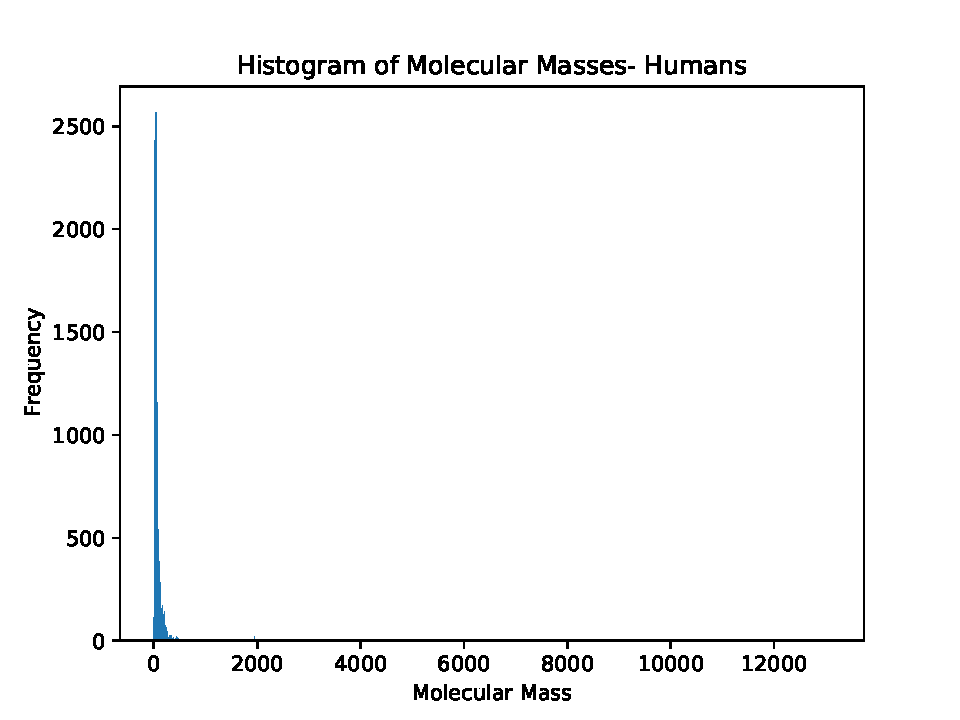
\includegraphics{human_mass.pdf}
\centering 
\end{figure}
\pagebreak 
\section{Problem 4}
The probability of having $0$ and $6$ is $$p^{3}q^{3}$$. 
The probability of having $1$ and $5$ is 
$$\binom{3}{1}p^{4}q^{2}+\binom{3}{1}p^{2}q^{4}$$
The probability of having $2$ and $4$ in one cell is
$$\binom{3}{2}p^{5}q^{1}+\binom{3}{2}p^{1}q^{5}+\binom{3}{1}\binom{3}{1}p^{3}q^{3}$$
The probability of having $3$ in one cell is
$$p^{6}+q^{6}+\binom{3}{1}\binom{3}{2}p^{2}q^{4}+\binom{3}{2}\binom{3}{1}p^{4}q^{2}$$
By substituting $p=0.5+x$, and minimizing using the least-squares method with respect to the experimental distribution, obtained value for p is $0.936093$.
Attached, is a scatter plot showing the deviation. Given that, there are only 6 molecules, and the error is about $0.007 \pm 0.001$ (for the non-zero values), I believe it's a good model. \newline
\begin{figure}
    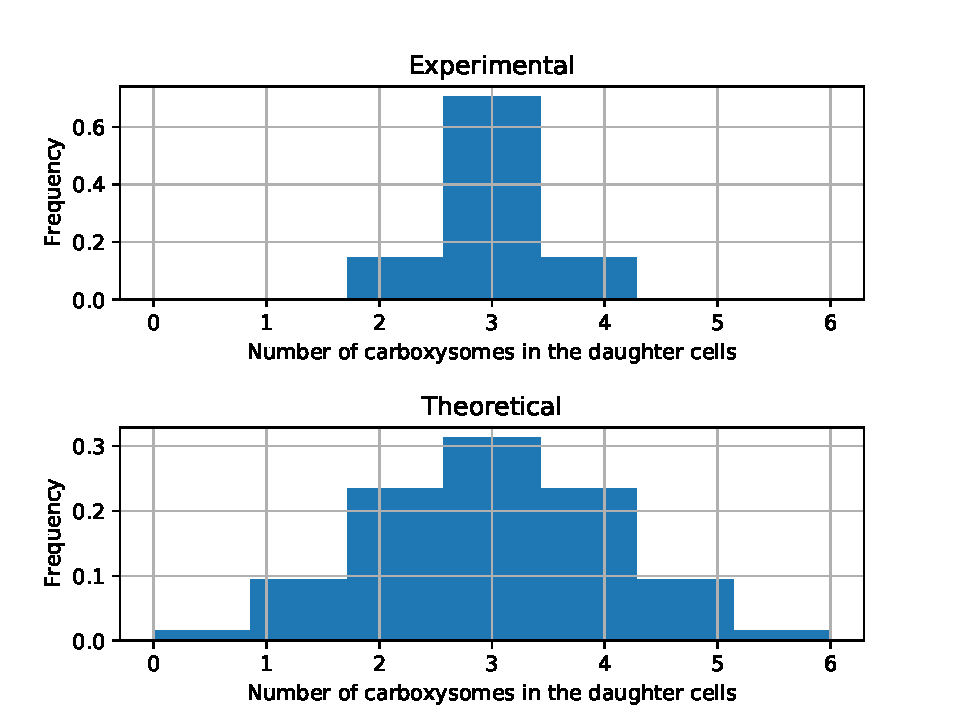
\includegraphics{q4.pdf}
    \centering 
\end{figure}
\begin{figure}
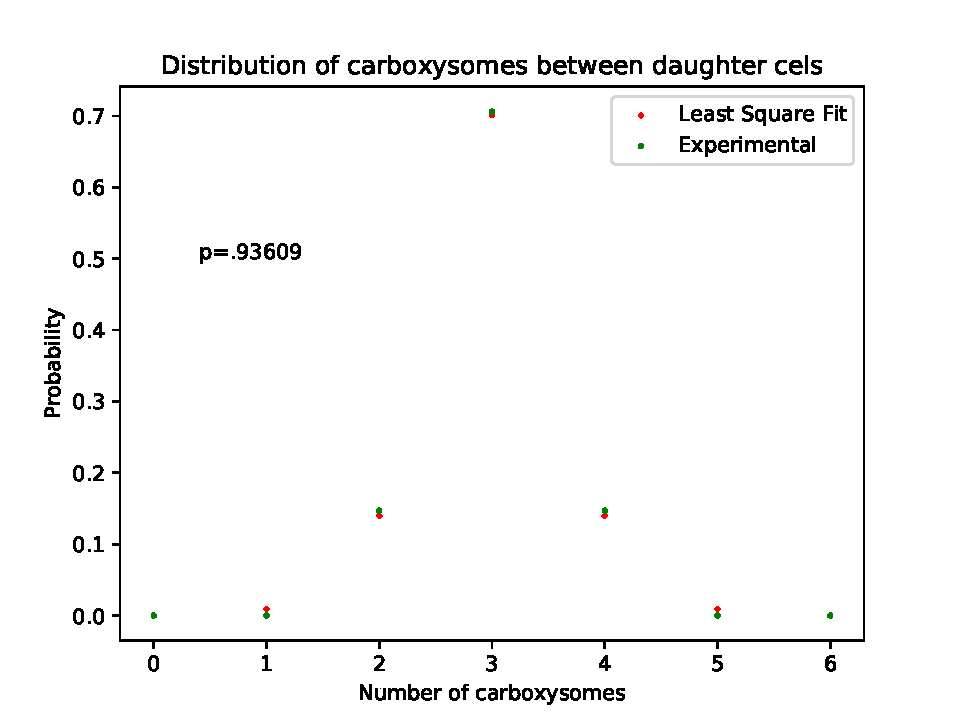
\includegraphics{q41.pdf}
\centering 
\end{figure}
\pagebreak
\section{Problem 5}
\begin{enumerate}[label=(\alph*)]
    \item There are $4^3$ possible ways of choosing the bases to form a triplet, each with the same probability. Therefore, $$p_{s}=\frac{3}{64}$$
	\item There are 64 possible codons. Three of these are not allowed(The stop codons), to form an ORF.Therefore, the number of acceptable possibilities is $(64-3)^{N}$.\newline
	Required probability is $\left(\frac{61}{64}\right)^{N}$.
	\item Codons are of length $3$ bases. Since, the DNA is circular, let us pick an arbitray base and call it the starting point, and label the bases as $$\dots x_{N-1}x_{N}x_{0}x_{1}x_{2}\dots$$
    Looking at the above sequence, we can see that the codons containing $x_{0}$ are
    \begin{align*}
        & x_{N-1}x_{N}x_{0} \\
        & x_{N}x_{0}x_{1} \\
        & x_{0}x_{1}x_{2} \\
    \end{align*} and their reverse(corresponding to either a clockwise read or an anti-clockwise read -- Also respectively, each codon corresponds to reading frames: $+2$,$+1$ and $+0$). Therefore, there are $6$ reading frames in total. 
    \item skip
    \item Take a look at the attached ipython notebook.
    \item The figures are placed at the end. 
    \item 1
    \begin{figure}
        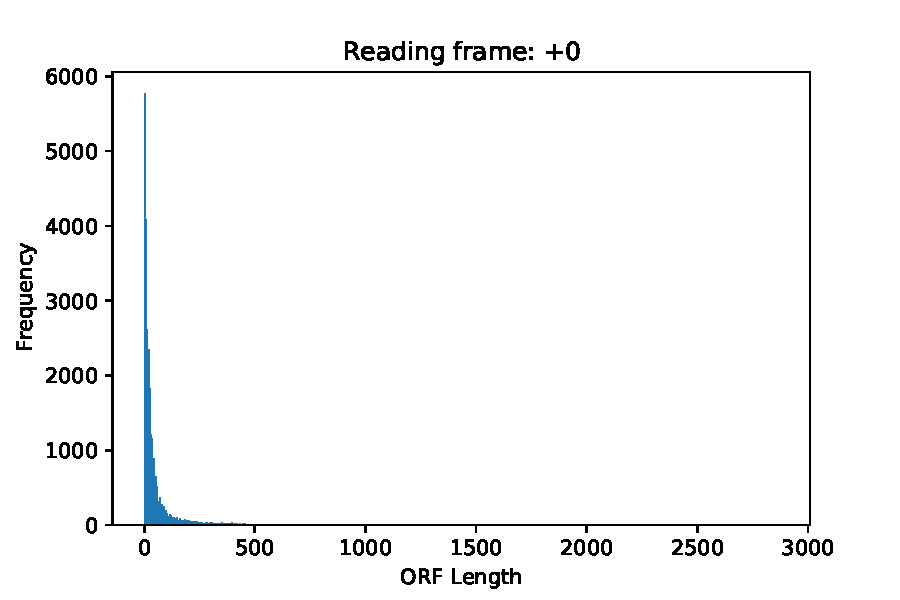
\includegraphics{q5f0.pdf}
        \centering
    \end{figure}
    \begin{figure}
        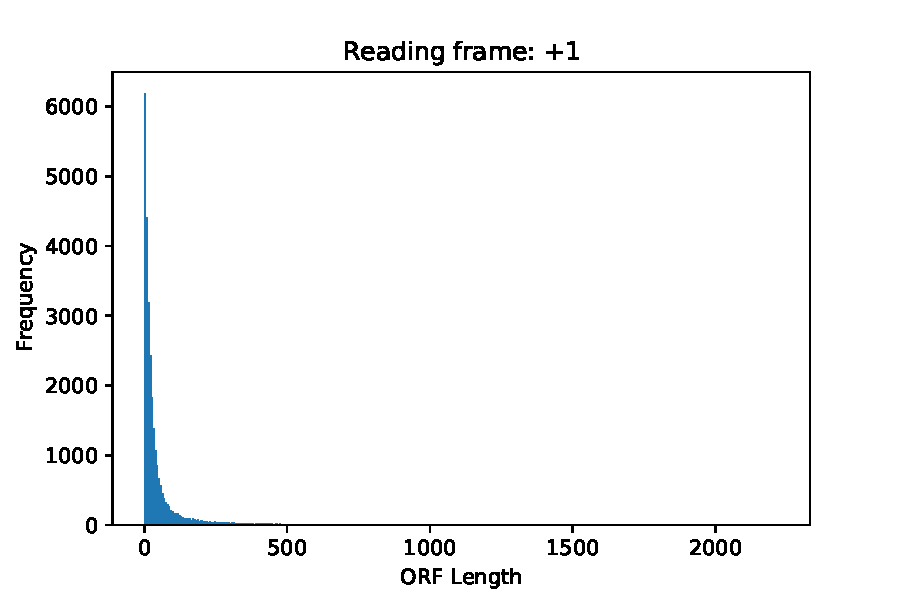
\includegraphics{q5f1.pdf}
        \centering
    \end{figure}
    \begin{figure}
        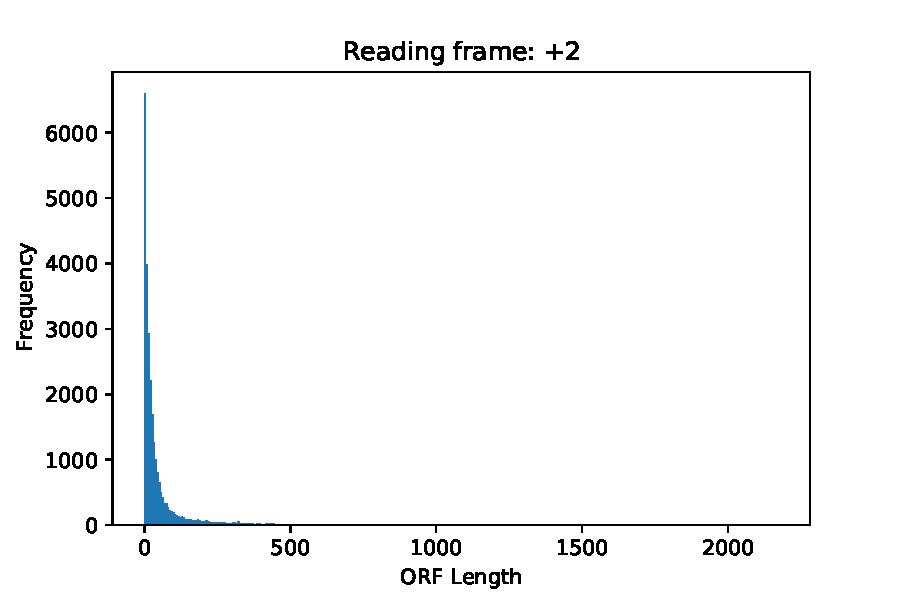
\includegraphics{q5f2.pdf}
        \centering
    \end{figure}
\end{enumerate}
\end{document}